% Template for ICIP-2015 paper; to be used with:
%          spconf.sty  - ICASSP/ICIP LaTeX style file, and
%          IEEEbib.bst - IEEE bibliography style file.
% --------------------------------------------------------------------------
\documentclass{article}
\usepackage{graphicx,listings,spconf,todonotes}

\title{Image Classification Using SIFT Features and Artificial Neural Network}

\name{Dan Chianucci, Peter Muller}
\address{Rochester Institute of Technology\\
	Computer Engineering Department}


\begin{document}
%\ninept
%
\maketitle
%
\begin{abstract}
In computer vision topics, classification is one of the more difficult actions that can be done with an image. Classification is the process of interpreting the contents of an image to sort it into one of several classes. In this experiment, SIFT, or Scale-Invariant Feature Transform, image features were extracted from images of the Caltech 101 data set. These features were quantized using K-means clustering, which were then used to train an artificial neural network (ANN) structure. For the limited dataset of 341 images, a 72.5\% accuracy in classification was achieved. It was expected that a combination of a larger dataset and more hidden layers in the ANN would help to improve accuracy in future experiments.
\end{abstract}
%
\section{Introduction}
\label{sec:intro}
\todo[inline]{Actual research into related works and the direction of our own experiment.}
%
\section{Methods}
\label{sec:methods}
As an overview of the experiment, several steps were taken. First, images from a single dataset were processed, and SIFT features were extracted from them. Preprocessing to normalize image intensities was not necessary because SIFT already accounted for these variations. An image compared with the same image, except for intensity variations, would still return the same SIFT features.

After every feature was collected from each image of the dataset, the data was quantized. K-means clustering was used to create bins for a histogram representation of the features. With a general structure that could be compared to for all images, the nearest-neighbor cluster centroids were used to count how many sift features appeared per histogram bin per image. These histograms gave the unique characteristics of each image class, which would be used for pattern recognition training in an artificial neural network.

A matrix of expected results was made for the training of an artificial neural network. In theory, the histograms of images in the same class should be very similar, so the ANN would be able to recognize these patterns and classify unknown images accordingly. Given these steps, the image classifications could be demonstrated.
%
\section{Experimental Setup}
\label{sec:expsetup}

In this experiment, five classes of images, trilobite, nautilus, scorpion, sea\_horse, and stegosaurus, were selected from the Caltech 101 image dataset\cite{LiFergusPerona04}. Because these images were all from the same dataset, no dataset bias was introduced like it would be if images from different datasets were used for classification. 

To begin the classification process, features were extracted from the five selected classes of images. For each image, SIFT features were collected into an overlying data structure which contained the SIFT features from all images. As mentioned previously, preprocessing of images was not required because the SIFT features would not change based on different image intensities.

After the collection of all SIFT features, K-means clustering was used to quantize the features database into a structure that individual image histograms would be compared to. For finding the best accuracy of the classifier, different K-values of 10, 20, 50, and 100 were considered. Because of the clustering, the mean centroids could be used to associate SIFT features of an individual image to the rest of the dataset. Using the nearest-neighbor centroid to the SIFT features of each individual image, histograms were calculated, denoting how many features were associated with a specific centroid. These histograms were used as inputs for the training and classification of images within the artificial neural network structure.

Of the 341 images investigated in this experiment, 239 images were used for training, 51 images were used for verification of the training, and 51 images were used for the actual classification experiment. Using the feature histograms from each image and a matrix of expected classifications, the artificial neural network was trained to identify and classify the different image classes. The Neural Net Pattern Recognition application from the Neural Network Toolbox in MATLAB was used for the training and creation of the ANN, which was used to retrieve the results of the classifications.

%
\section{Results}
\label{sec:results}
Upon training the ANN, it was apparent that parameters of the experiment had to be altered to achieve the highest possible accuracy of classification. After fixing the number of nodes in the hidden layer of the neural network to 20 nodes, the only variable to adjust was the number of bins in the histograms generated using the K-means quantization. The following figures show a comparison of the classification accuracies of different K-values used during the quantization stage in the form of confusion matrices. Figure \ref{fig:k10} shows the confusion matrices of the classification with a K-value of 10, Figure \ref{fig:k20} shows the matrices with K=20, Figure \ref{fig:k50} shows them with K=50, and Figure \ref{fig:k100} shows the matrices with K=100. To visualize this data, receiver operating characteristic, or ROC, curves were created, which show the true positive rate, the rate at which images correctly mapped to their classes, in comparison to the false positive rate, the rate at which images are falsely classified into different classes than their own class. These curves are shown in Figures \ref{fig:r10}, \ref{fig:r20}, \ref{fig:r50}, and \ref{fig:r100}.
%
\begin{figure}[Ht]
\centering
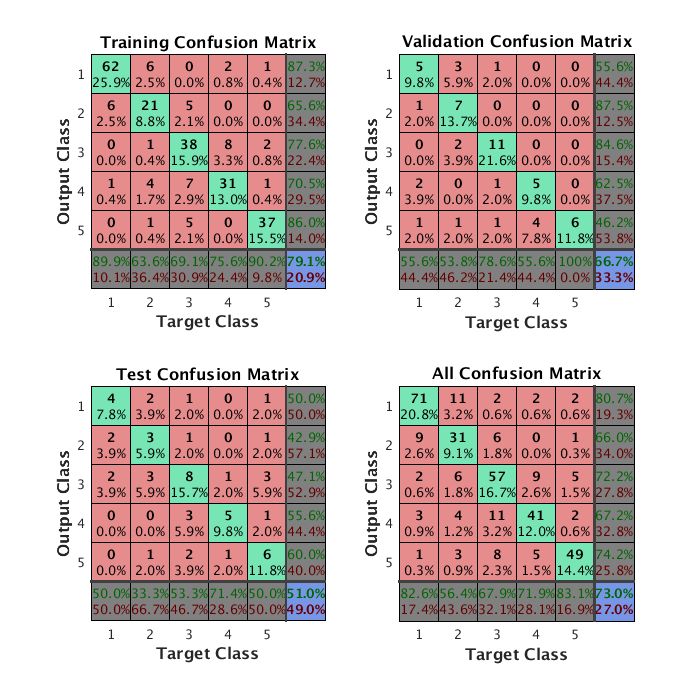
\includegraphics[scale=0.5]{Figures/Metrics/conf_k10}
\caption{Confusion matrices with K=10.}
\label{fig:k10}
\end{figure}
\begin{figure}[Ht]
\centering
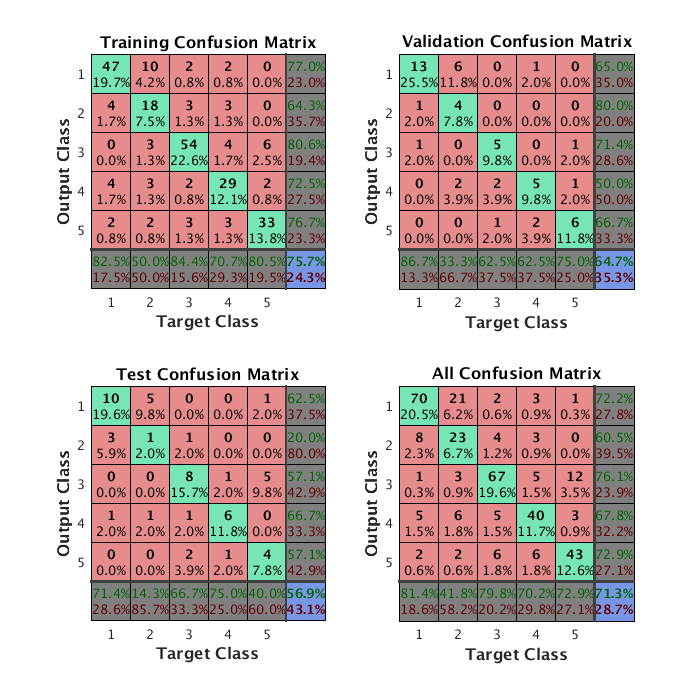
\includegraphics[scale=0.5]{Figures/Metrics/conf_k20}
\caption{Confusion matrices with K=20.}
\label{fig:k20}
\end{figure}
\begin{figure}[Ht]
\centering
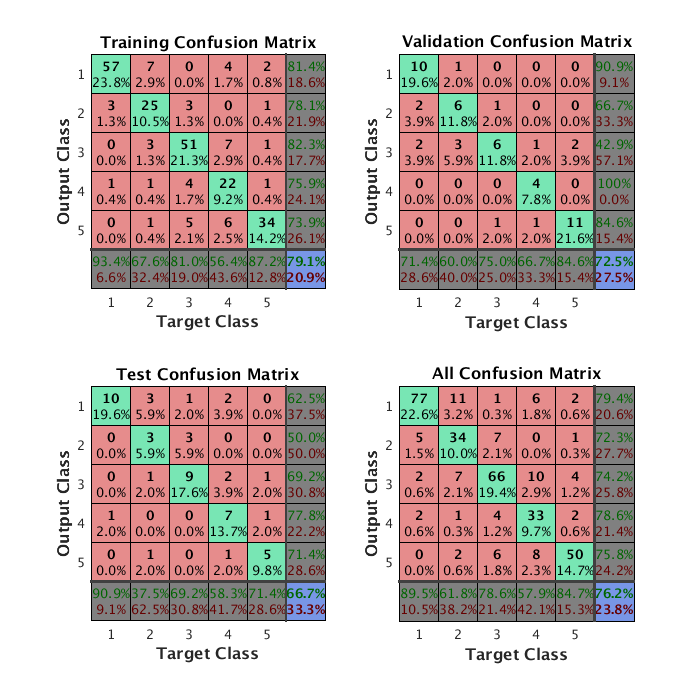
\includegraphics[scale=0.5]{Figures/Metrics/conf_k50}
\caption{Confusion matrices with K=50.}
\label{fig:k50}
\end{figure}
\begin{figure}[Ht]
\centering
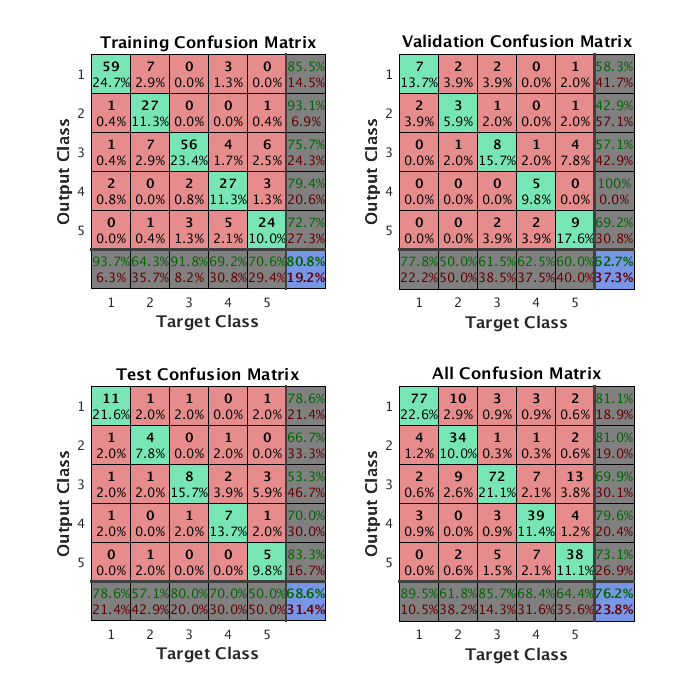
\includegraphics[scale=0.5]{Figures/Metrics/conf_k100}
\caption{Confusion matrices with K=100.}
\label{fig:k100}
\end{figure}
\begin{figure}[Ht]
\centering
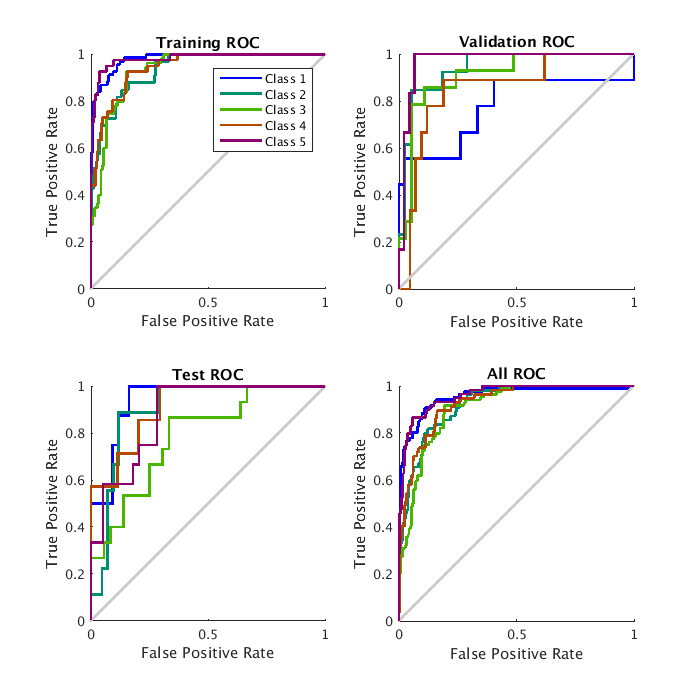
\includegraphics[scale=0.5]{Figures/Metrics/roc_k10}
\caption{ROC curves with K=10.}
\label{fig:r10}
\end{figure}
\begin{figure}[Ht]
\centering
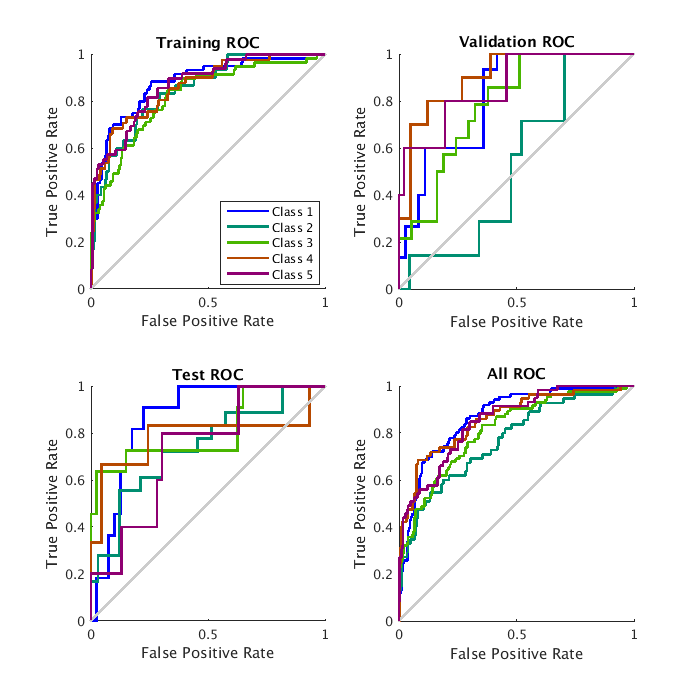
\includegraphics[scale=0.5]{Figures/Metrics/roc_k20}
\caption{ROC curves with K=20.}
\label{fig:r20}
\end{figure}
\begin{figure}[Ht]
\centering
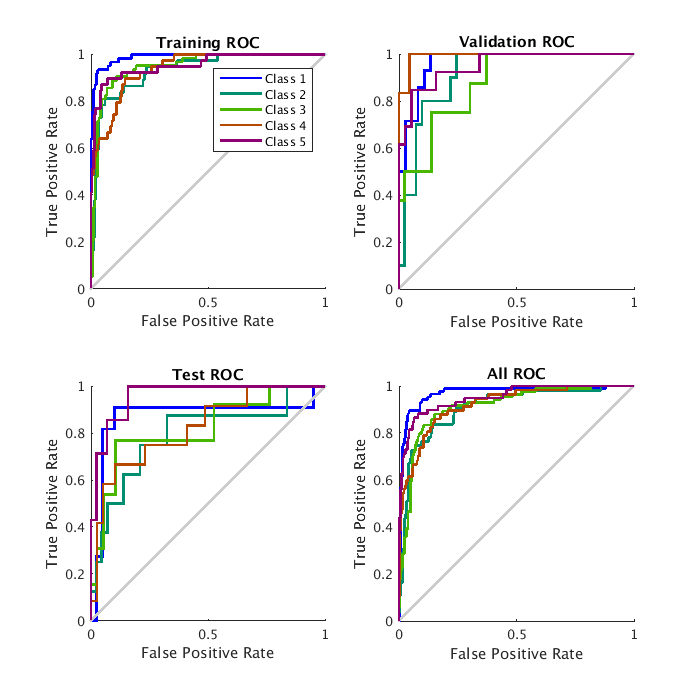
\includegraphics[scale=0.5]{Figures/Metrics/roc_k50}
\caption{ROC curves with K=50.}
\label{fig:r50}
\end{figure}
\begin{figure}[Ht]
\centering
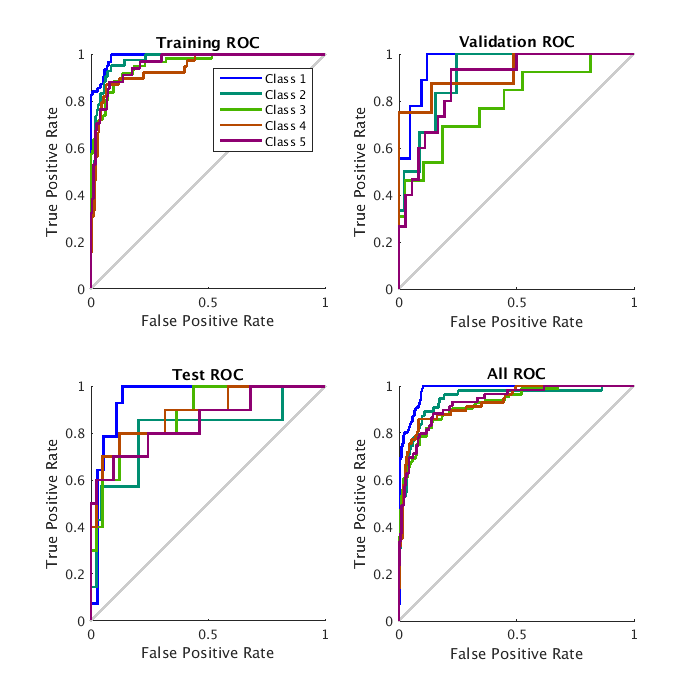
\includegraphics[scale=0.5]{Figures/Metrics/roc_k100}
\caption{ROC curves with K=100.}
\label{fig:r100}
\end{figure}
%

As supported by these figures, increasing the K-value when quantizing the SIFT features increased the accuracy of the system. The rate of true positives compared to false positives was greater in the larger values of K than in the smaller values.

Next, since the system accuracy was verified, the resulting images could be retrieved for comparison. For each class, the best results, as determined by the classification probabilities of the artificial neural network, and the worst results, false positives with high classification probabilities and false positives with low classification probabilities, are shown. Table \ref{tab:results} shows the comparison of these images for each class.

\begin{table}[Ht]
\caption{Best and worst results of image classification.}
\label{tab:results}
\begin{tabular}{| c | c | c | c |}
\hline
Class & Best Match & False Positive & False Positive \\
 & & with & with \\
 & & High Probability & Low Probability \\
\hline
trilobite &
\vspace{0cm}\includegraphics[scale=.1]{"Figures/Best Matches/bestmatch_c1"} &
\vspace{0cm}\includegraphics[scale=.1]{"Figures/False Matches/class_1_most_sure_wrong"} &
\vspace{0cm}\includegraphics[scale=.1]{"Figures/False Matches/class_1_least_sure_wrong"} \\
\hline
nautilus &
\vspace{0cm}\includegraphics[scale=.1]{"Figures/Best Matches/bestmatch_c2"} &
\vspace{0cm}\includegraphics[scale=.1]{"Figures/False Matches/class_2_most_sure_wrong"} &
\vspace{0cm}\includegraphics[scale=.1]{"Figures/False Matches/class_2_least_sure_wrong"} \\
\hline
scorpion &
\vspace{0cm}\includegraphics[scale=.1]{"Figures/Best Matches/bestmatch_c3"} &
\vspace{0cm}\includegraphics[scale=.1]{"Figures/False Matches/class_3_most_sure_wrong"} &
\vspace{0cm}\includegraphics[scale=.1]{"Figures/False Matches/class_3_least_sure_wrong"} \\
\hline
sea\_horse &
\vspace{0cm}\includegraphics[scale=.1]{"Figures/Best Matches/bestmatch_c4"} &
\vspace{0cm}\includegraphics[scale=.1]{"Figures/False Matches/class_4_most_sure_wrong"} &
\vspace{0cm}\includegraphics[scale=.1]{"Figures/False Matches/class_4_least_sure_wrong"} \\
\hline
stegosaurus &
\vspace{0cm}\includegraphics[scale=.1]{"Figures/Best Matches/bestmatch_c5"} &
\vspace{0cm}\includegraphics[scale=.1]{"Figures/False Matches/class_5_most_sure_wrong"} &
\vspace{0cm}\includegraphics[scale=.1]{"Figures/False Matches/class_5_least_sure_wrong"} \\
\hline
\end{tabular}
\end{table}
%
\section{Discussion}
\label{sec:discussion}
One of the major factors of the accuracy of a neural network classifiers was the amount of training data available for it to consume. Because only five classes were chosen for processing, that greatly reduced the number of images that could be used. Considering other implementations of neural networks, the lack of a large dataset was compensated by using a large number of nodes in the hidden layer within the ANN itself. This implementation used 20 nodes for the hidden layer. Further research could determine the optimal number of nodes to use in this type of situation. 

Because of the fixed number of nodes in the hidden layer, the K-value, used for clustering, was varied to achieve the greatest accuracy of the network, given little training data to work with. As shown in Figures \ref{fig:k10}, \ref{fig:k20}, \ref{fig:k50}, and \ref{fig:k100}, the K-value of 100 gave the highest accuracy. Considering the visuals of the ROC curves in Figures \ref{fig:r10}, \ref{fig:r20}, \ref{fig:r50}, and \ref{fig:r100}, ideal classifications would have a true positive rate of 1 at the false positive rate of 0. Although the experimental ROC curves do not achieve the ideal conditions, they still perform with a high accuracy.

After determining the most accurate model for data quantization and classification, the image results were then retrieved. Table \ref{tab:results} shows the best results, which are the images with the highest probability that they were in the correct class, and the worst results, which are the images which were wrongly classified with high and low probabilities of being in that particular class. It can be seen that similar image structures were grouped together, especially curves, which several of the images had in common. In the sea\_horse class, the same false positive shows up as the best result and the false positive with a high probability. This is because this particular image outweighed other probabilities, including those of true positives for the sea\_horse class. For every other class, the best match was within the same class.

Considering the amount of data used in this experiment, the classifier accuracy was moderately high, but there were opportunities for improvements. A simple way to increase the classifier accuracy would be to train with more data. The data subset used in this experiment only contained 341 images, but if each class had more data to train on, the neural network would have been able to adjust its weights to the greater data, which could have increased classification accuracy.

Other ways of improving this implementation would involve modifying the ANN itself. By converting the artificial neural network into a deep belief network, higher accuracies could be experienced. This was simply a matter of adding more hidden layers to the ANN structure. In addition, more research could be done to see the effects of adding more nodes to the existing hidden layer. For the purposes of this experiment, the value was fixed at 20, but its effects were not explored any further in this context.

% References should be produced using the bibtex program from suitable
% BiBTeX files (here: refs). The IEEEbib.bst bibliography
% style file from IEEE produces unsorted bibliography list.
% -------------------------------------------------------------------------
\bibliographystyle{IEEEbib}
\bibliography{refs}

\newpage
\appendix
\section{Appendix: Source Listing}
\label{sec:source}
\todo[inline]{include matlab code.}
\lstinputlisting[language=Matlab, frame=single, caption=startup.m]{../startup.m}
\lstinputlisting[language=Matlab, frame=single, caption=run\_script.m]{../run_script.m}
\lstinputlisting[language=Matlab, frame=single, caption=calculate\_features.m]{../calculate_features.m}
\lstinputlisting[language=Matlab, frame=single, caption=gen\_train\_data.m]{../gen_train_data.m}
\lstinputlisting[language=Matlab, frame=single, caption=sift\_descriptor.m]{../sift_descriptor.m}
\lstinputlisting[language=Matlab, frame=single, caption=read\_gray.m]{../read_gray.m}
\lstinputlisting[language=Matlab, frame=single, caption=train\_nn.m]{../train_nn.m}


\end{document}
